% Project Specification
\begin{figure*}[t]
  \begin{minipage}[t]{0.33\textwidth}
    \centering
    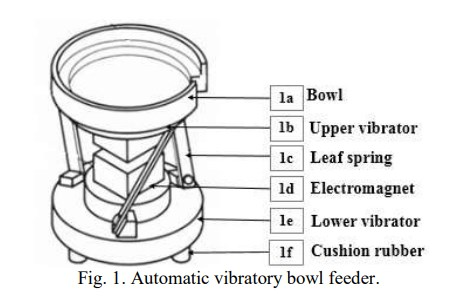
\includegraphics[width=\textwidth,height=5cm, keepaspectratio]{imgs/articles/feeder.jpg}
    \caption{VBF\cite{nam2019design}}
    \label{fig:feeder}
  \end{minipage}
  \hfill
  \begin{minipage}[t]{0.33\textwidth}
      \centering
      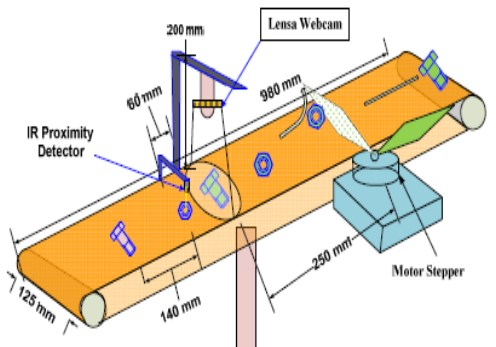
\includegraphics[width=\textwidth,height=5cm, keepaspectratio]{imgs/articles/conveyor.jpg}
      \caption{Conveyor Belt\cite{Dhenge2013MechanicalNS}}
      \label{fig:conveyor}
      \end{minipage}
  \hfill
  \begin{minipage}[t]{0.33\textwidth}
    \centering
    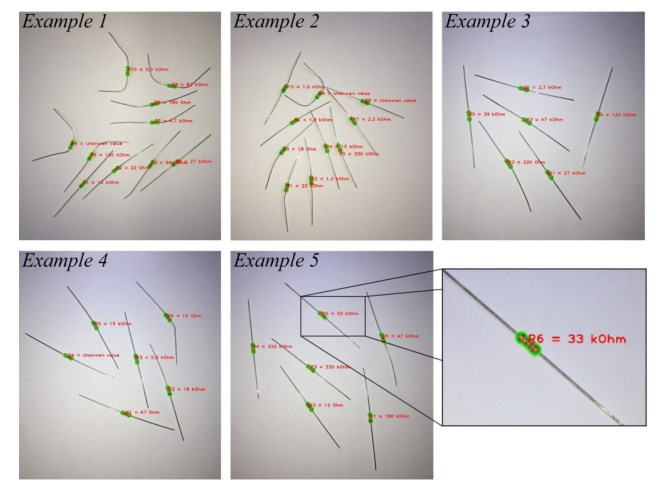
\includegraphics[width=\textwidth,height=5cm, keepaspectratio]{imgs/articles/resistordata.jpg}
    \caption{Resistor Test Set\cite{8939034}}
    \label{fig:resistordata}
  \end{minipage}
\end{figure*}

\section{Project Specification}
\label{sec:project-specification}
This project aims to solve the problem of electronic waste and cluttered workspaces in the Level 1 Labs
by developing an automated system for identifying and sorting electronic components.

It aims to do so by employing state-of-the-art computer vision techniques to classify various electronic components,
and then sort them into designated bins. The project's deliverables are as follows:
\begin{mylist}
  \item A computer vision system for component identification
  \item An interface from which to observe and control the system's state
  \item A semi-automated sorting mechanism
  \item Potentially, full automation of the sorting process or additional features like IC testing
\end{mylist}
\noindent
After an initial consultation with my supervisor Dr. Stott and a visit to the Level 1 Labs to discuss the project, I received a sample
of the different electrical components that were commonly used, which are the following:
\begin{multicols}{2}
  \begin{mylist}
    \item Resistors
    \item Capacitors
    \item Ceramic Capacitors
    \item Inductors
    \item Diodes
    \item MOSFETs
    \item Transistors
    \item LEDs
    \item Wires
    \item ICs
  \end{mylist}
\end{multicols}

\noindent
For this initial stage of the project, the focus is on developing the foundation of the system that the project
will be built upon so that the development of the various systems can be done independently, in parallel, and in such a way that each system
is modular and easily extensible. For this reason, the project is split into three stages:
\begin{mylist}
  \item Initial development of a computer vision system for component identification
  \item Integration of a semi-automated sorting mechanism
  \item Potentially, full automation of the sorting process or additional features like IC testing
\end{mylist}
This approach was taken to allow me to set defined goals to ensure that the project is always working towards a deliverable product.
Each stage extends the previous stage, so the project can be considered as a series of smaller projects. 
